%% $Id: parallel.tex,v 1.23 2007/04/22 13:50:54 benkirk Exp $
\chapter{Parallel Issues and Data Structures\label{chap:parallel}}

%%%%%%%%%%%%%%%%%%%%%%%%%%%%%%%%%%%%%%%%%%%%%%%%%%%%%%%%%%%%%%%%%%%%%%%%%%%%%%
Adaptive simulation techniques necessarily produce dynamic simulations which have historically been difficult to implement effectively on parallel computers. This chapter continues from the AMR software framework considerations of Chapter~\ref{chap:amr} to address particular issues which arise on parallel, high-performance computers.  We begin with a brief overview of parallel architectures and a discussion of their importance.  Next the particular challenges for AMR schemes in this setting are described, along with a discussion of how particular data structures may be used to help ease the implementation of adaptive methods on parallel architectures.

%%%%%%%%%%%%%%%%%%%%%%%%%%%%%%%%%%%%%%%%%%%%%%%%%%%%%%%%%%%%%%%%%%%%%%%%%%%%%%
\section{Parallel Computing}
\subsection{Background}
Parallel computing has become the \emph{de facto} method used to achieve high-performance, large-scale simulation. These parallel machines have largely replaced specialized vector machines for scientific computing, due in part to their price per-performance benefit.  %Gropp et. al draw an enlightening analogy: ``To pull a bigger wagon, it is easier to add more oxen than to grow a gigantic ox.''~\cite{gropp_using_mpi}  Such it is with parallel computing.

In the 1970's and '80's scientific computing represented a significant portion of the computer market.  Specialty machines which used vector processing units, produced by companies such as IBM and Cray, were common.  From the mid-1990's to present day, however, the landscape has changed remarkably.  Scientific computing now represents only a small fraction of the computer market.  Rather than driving technology innovations, the scientific computing market now finds itself adapting hardware developed largely for other fields.

Parallel computing is one way in which scientific computing has dealt with this changing landscape.  In general, the distinguishing feature of a parallel architecture is that each processor is connected to its own memory resources which cannot be seen by other processors.
\begin{figure}[hbtp]
  \begin{center}
    \subfigure[shared memory]{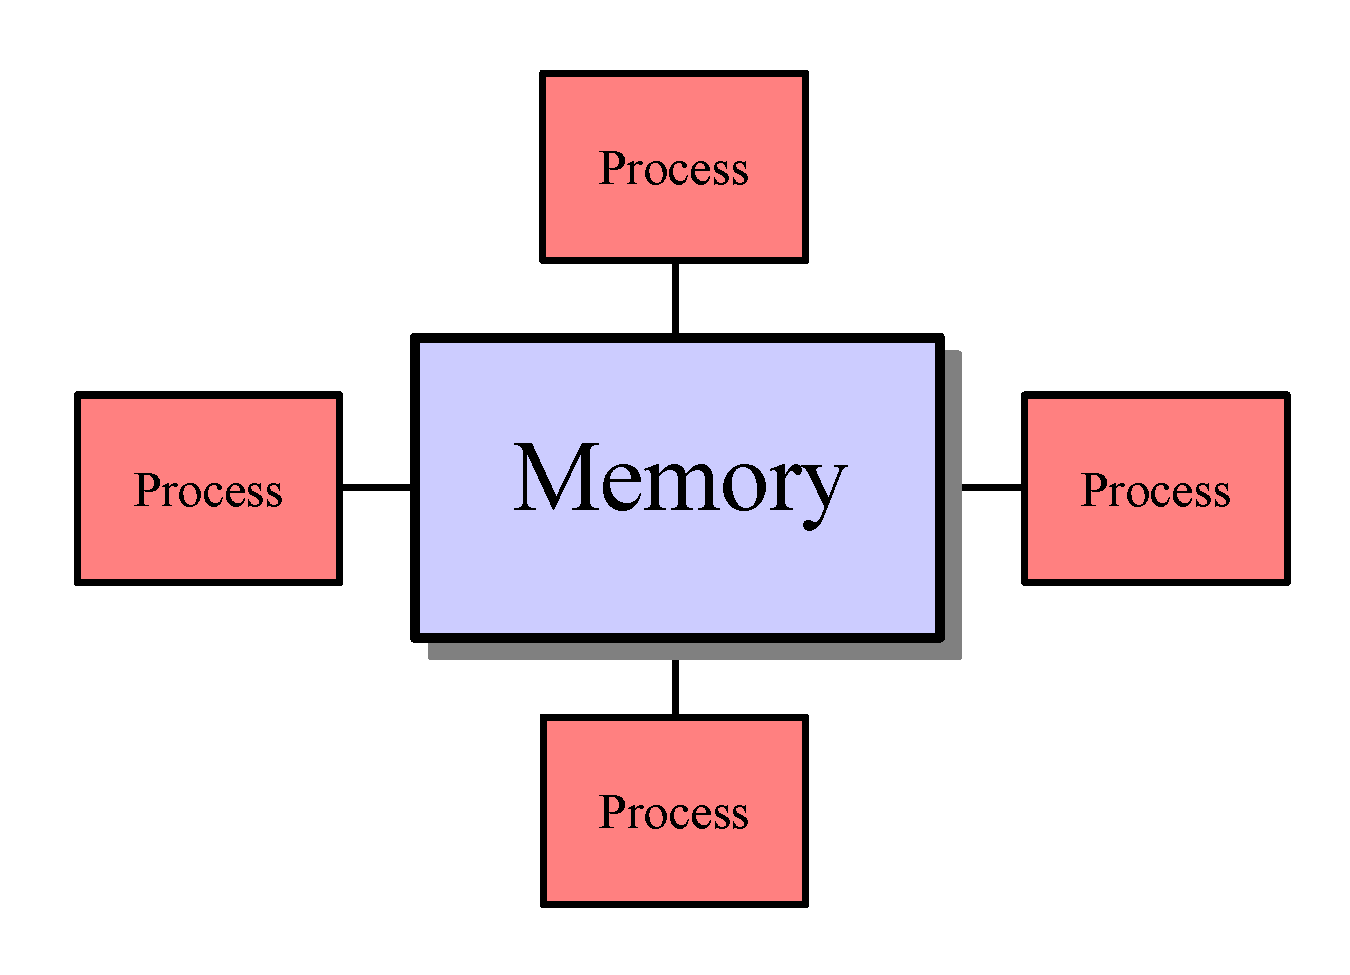
\includegraphics[height=.4\textheight]{figures/parallel_architectures/shared}} \\
    \subfigure[distributed memory]{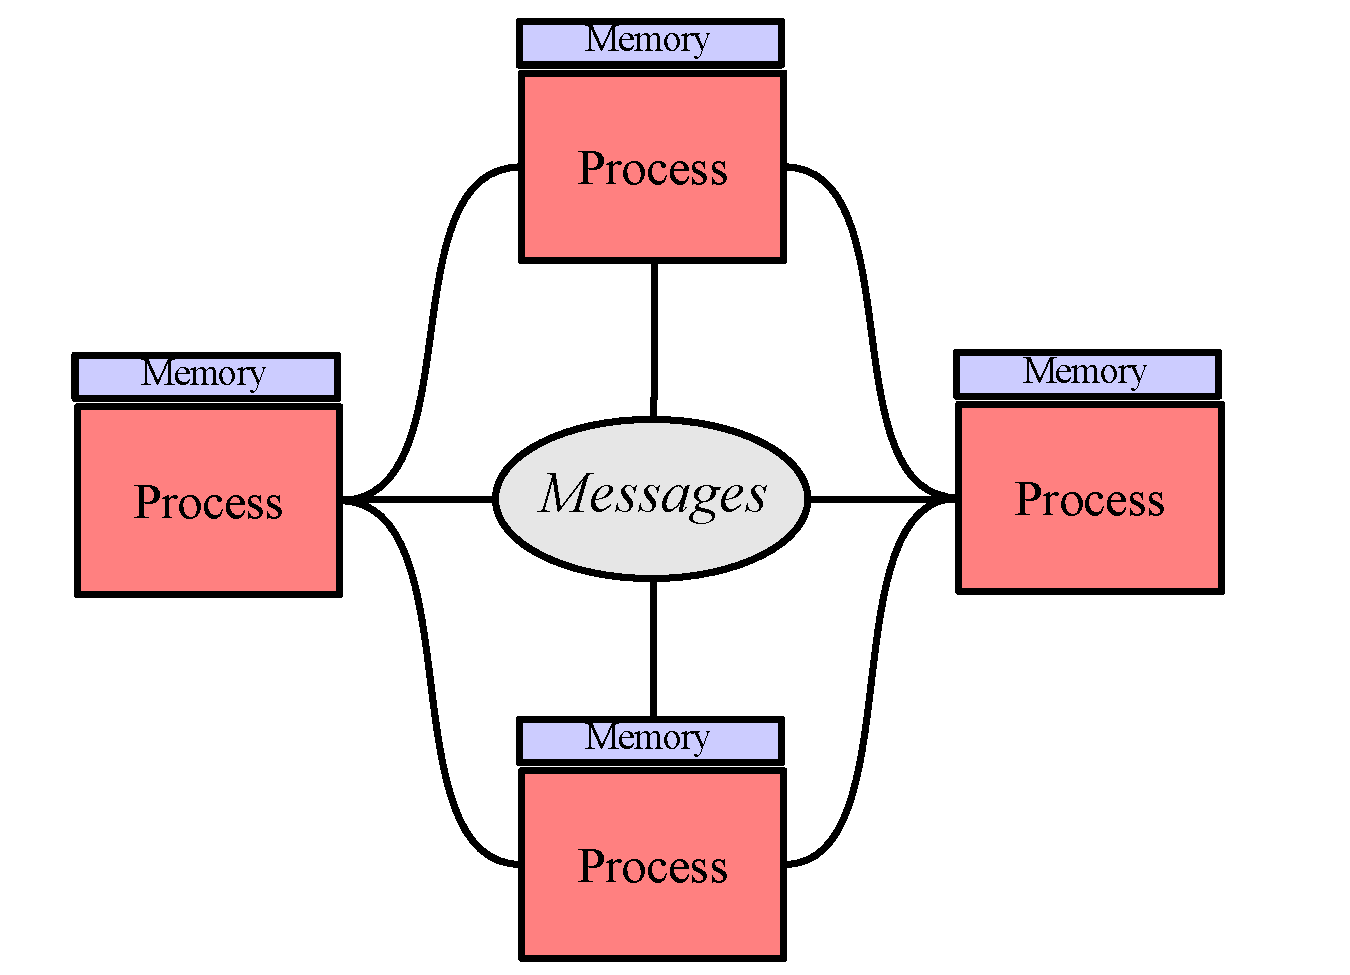
\includegraphics[height=.43\textheight]{figures/parallel_architectures/distributed}}
      \caption{Shared and distributed-memory parallel architectures.\label{fig:shared_dist}}
  \end{center}
\end{figure}
This \emph{distributed memory} paradigm introduces particular complications in the development of parallel algorithms, as some form of message passing must be used to enable communication between collaborating processors.  This is in contrast to \emph{shared memory} machines, in which each processor has access to a large, global pool of memory. The two basic architectures are represented schematically in Figure~\ref{fig:shared_dist}. Parallelizing software for shared memory architectures is simpler than in the distributed case because data can be immediately accessed by all processors.  

The parallel architecture paradigm provides one strong benefit: scalability. The vast majority of the world's fastest computers as of the time of this writing are massively parallel machines comprised of $\mathcal{O}(10,000)$ commodity server-class machines.\footnote{\url{http://www.top500.org},\mbox{ } January 2007.}

%\clearpage
\subsection{Implications for Mesh-based Simulations}
Mesh-based simulation techniques approximate the solution to a set of governing equations by solving a discrete representation of the problem.  Discretization is performed with a mesh that describes the physical domain of interest.  For parallelization, a computational mesh can be decomposed into a number of subdomains which are each assigned to one of the processors used in the simulation.  This \emph{domain decomposition} approach is common and will be the focus of Section~\ref{sec:dd}.

Of course, some form of communication is required between processor subdomains in this approach.  The amount of data required to be communicated between processors to enable this approach is highly dependent on the partitioner used to create the domain decomposition and on the choice of data structures used in the software implementation, as this drives which data are required from adjacent processors.  Some key aspects of the data structures used in this work will be discussed in Section~\ref{sec:dsr} with an emphasis on how they influence the parallel implementation.

In general, implicit techniques require that a linear system be constructed and solved as part of the solution algorithm.  In parallel the construction of this system is largely unchanged from the serial case.  The solution of the system, however, must account for the distributed nature of the machine.  Specifics regarding parallelization within finite element simulations is the focus of Section~\ref{sec:parallel_issues}.



%%%%%%%%%%%%%%%%%%%%%%%%%%%%%%%%%%%%%%%%%%%%%%%%%%%%%%%%%%%%%%%%%%%%%%%%%%%%%%
\section{Domain Decomposition\label{sec:dd}}
A non-overlapping domain decomposition approach is used in
\libMesh{} to achieve data distribution on parallel computers as shown
in Figure~\ref{fig:orbiter_dd}~\cite{carey_gridbook}.  The discrete
domain $\Omega_h$ is partitioned into a collection of subdomains
$\left\{\Omega_h^p\right\}$ such that $\bigcup\Omega_h^p=\Omega_h$ and
$\bigcap\Omega_h^p=\emptyset$. Each subdomain $\Omega_h^p$ is
assigned to an individual processor.
\begin{figure}
  \begin{center}
    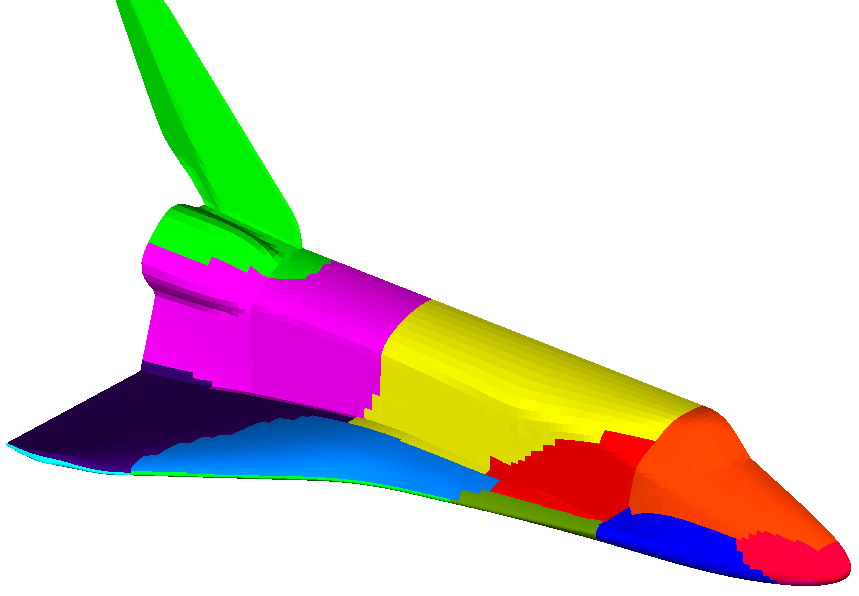
\includegraphics[width=.7\textwidth]{figures/domain_decomposition/orbiter_surface}
    \caption{Element-based domain decomposition of a surface mesh
      into 16 subdomains\label{fig:orbiter_dd}}
  \end{center}
\end{figure}
Two primary metrics in judging the quality of a partitioning scheme's computation and communication load balance are (1) the
subdomain mesh size and (2) the number of ``edge cuts'' in the resulting
partition.  For a mesh composed of a single type of element,
each subdomain should contain essentially an equal number of elements so that the
computational work is load balanced across all available processors.  The
edge cut metric, on the other hand, is related to the
interprocessor communication required by the parallel solver.
For an overview of several domain decomposition strategies
that are available see~\cite{iqbal_carey_2005,ZoltanOverviewArticle}.

In problems with high-resolution static meshes, the partitioning is
only performed once.  In such cases, a high-quality 
partition which simultaneously minimizes both the subdomain's
size and edge-cut metrics may be desirable, even though it may be
relatively expensive.  For adaptive refinement and coarsening 
applications where the steady-state solution is of interest, it is
frequently the case that one begins with a coarse mesh at the root
level and selectively refines towards a near-optimal mesh with
little coarsening. It is obvious that an initially balanced partition
may become unbalanced very rapidly, leading to parallel computational
inefficiencies. Consequently, the mesh typically requires frequent
repartitioning during the AMR process. In this case a less expensive partitioning scheme may be desirable as it will be used repeatedly.
The development of optimal
schemes for
repartitioning that can take advantage of a prior partition in a
parallel AMR setting is still an open research
issue~\cite{iqbal_carey_2005}.

In \libMesh{} we partition by default using the recursive scheme
provided by METIS for coarse parallel granularity when the number of selected partitions $n_p \leq8$,
and with the k-way scheme otherwise~\cite{karypis:metis}.  A space filling
curve partitioning algorithm is also available, as is an interface to
ParMETIS.  The frequency of repartitioning needed will, in general,
depend on the evolving imbalance.  Currently, repartitioning is done
every time the mesh changes (i.e. every time refinement or coarsening
occurs).  Profiling suggests that this technique is not overly
inefficient for typical applications, but it could be very slow for
large-scale problems, and clearly it is unnecessary if the refinement
scheme selects only a small number of elements to be refined and
coarsened.  %(FIXME: elaborate here?)

\enlargethispage{-\baselineskip}
Another issue that must be considered is the subset of the AMR tree on
which the partitioning algorithm acts. Typically, the partitioning
algorithm is applied to all the active elements (i.e., the leaves of
the AMR tree) so that the resulting computational load is well balanced.  However, this approach involves calling
the partitioning algorithm on a large subset of the AMR tree, while it may
be sufficient to partition based on a coarser level and simply assign
all the children of these coarse level elements to the same processor.
Due to the parallel implementation of the \texttt{Mesh} discussed in
Section~\ref{sec:parallel_issues}, we do not (yet) consider the
possibility that accessing an ancestor element would require
off-processor communication.  In such a scenario, one would need to
ensure that repeated refinement and coarsening of the same region of the mesh 
did not lead to excessive communication overhead, perhaps by ensuring
that a local synchronized copy of an element's parent is always available.



%%%%%%%%%%%%%%%%%%%%%%%%%%%%%%%%%%%%%%%%%%%%%%%%%%%%%%%%%%%%%%%%%%%%%%%%%%%%%%
\section{Data Structures -- Parallel Aspects\label{sec:dsr}}
This section describes several of the key \libMesh{} data structures
which are important for parallel implementation.  The discussion
focuses on basic functionality, possible extensions, and the reasoning
behind certain design decisions in the context of parallel computing.
Algorithms that are central to the library's functionality are also
described.

\subsection{Element Hierarchy}
The refinement hierarchy and recursive constraint application procedure described in Section~\ref{sec:amr_data_structures} was chosen because it exploits data locality and minimizes the amount of inter-processor communication required to generate element constraints.

In general, the refined mesh will no longer be well-balanced across all
processors, and dynamic repartitioning (and possibly data
redistribution) is required.  The frequency of the dynamic
repartitioning process will influence the parallel performance of the
application.  The optimal repartitioning frequency will depend on the
relative computation/communication cost of the parallel system and the
solution algorithm employed.  To minimize the computational overhead incurred it is desirable that the entire refinement tree for a given root element reside in local memory.


\subsection{Degrees of Freedom\label{sec:dof_distribution_parallel}}
The domain decomposition approach described earlier assigns disjoint
groups of elements to individual processors.  This allows the
element-based degrees of freedom to be assigned uniquely to the
processor which owns the element, but requires some shared
distribution of vertex, edge, and face degrees of freedom which reside on subdomain boundaries.
Figure~\ref{fig:dofs_dd} illustrates the approach which is used in the
library.
\begin{figure}[hbtp]
  \begin{center}
    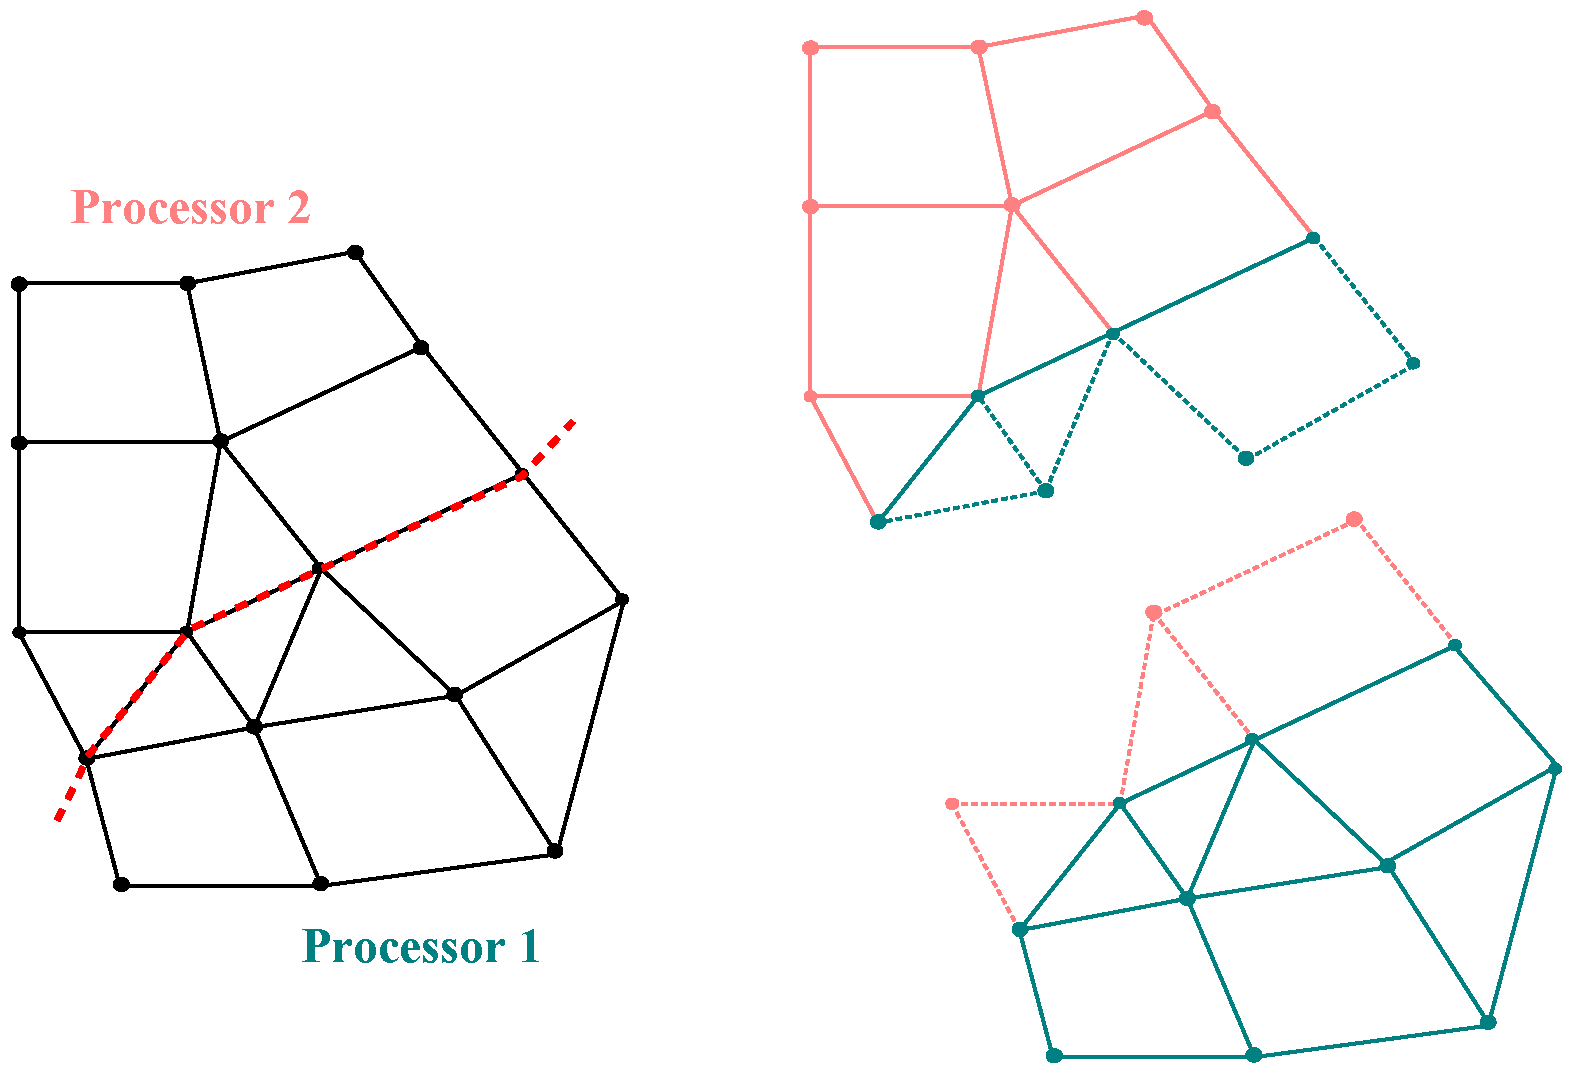
\includegraphics[width=\textwidth]{figures/data_structures/dofs}
    \caption{Element partitioning \& degree of freedom distribution\label{fig:dofs_dd}}
  \end{center}
\end{figure}

In this approach, any degrees of freedom on the border
between subdomains are owned by the processor of lowest
global rank.  This is evident from the figure, where the nodes on the
shared interface have been assigned to processor~1.

This approach for assigning degrees of freedom to processors also fits
well with the sparse matrix partitioning scheme employed in the underlying linear solver, in which  complete rows of the sparse matrix are assigned to individual
processors~\cite{petsc_manual}.  This is the natural matrix
decomposition that results from the degree of freedom distribution
depicted in Figure~\ref{fig:dofs_dd}.



%%%%%%%%%%%%%%%%%%%%%%%%%%%%%%%%%%%%%%%%%%%%%%%%%%%%%%%%%%%%%%%%%%%%%%%%%%%%%%
\section{Parallelization in Finite Element Simulations\label{sec:parallel_issues}}
\enlargethispage{-\baselineskip}
Parallelism in \libMesh{} is present at the matrix assembly and linear
algebra levels.  On distributed memory machines, such as PC clusters,
a complete copy of the mesh is maintained independently on each
processor. This design decision currently limits practical 3D
applications to 
the order of 128 processors because of the storage overhead associated with
storing the global mesh.  Nevertheless, a remarkable number of 3D
applications have been successfully solved using this implementation.
Fully parallel mesh data structures must contend with load balancing issues, however these issues are mitigated by keeping a copy of the mesh on each processor. The recent proliferation of hybrid distributed/shared
memory architectures, such as PC clusters with multi-core CPUs, 
suggests that corresponding parallel codes should include
% likely cause us to take a closer look at this design and investigate
% hybrid parallel programming paradigms such as
combined message passing and multithreading models.  While a complete
parallelization of the global mesh is not attempted in the present
work, Section~\ref{sec:parallelization_strategy} will outline the
approach which is intended to be pursued as future work.
 
One major goal of the library is to shield end-users from the
complexity of parallel programming, allowing them instead to focus on
the physics they are modeling.  The vision is that users develop and
debug applications on serial machines and then move seamlessly to
parallel architectures for large-scale simulations.  To achieve this
goal the library hides parallel communication from the user, so
basic message passing calls, for example, are not required at the user-level in most applications.

A case in point is the simple act of reading a mesh from disk.  The
user simply instantiates a \texttt{Mesh} object and calls its \texttt{read()}
member function.  This is a trivial operation from the user's point of
view, consisting of only two lines of code.  These two lines of code
are then executed on every processor in a parallel simulation, causing
a chain of events in which processor~1 actually reads the mesh from disk and broadcast the data
to the remaining processors.  This level of abstraction is common in
many numerical libraries (e.g. \PETSc{}) and provides encapsulation of
the library implementation so as not to affect user code.

\subsection{Data Dependencies}
The parallel degree of freedom distribution discussed in
Section~\ref{sec:dof_distribution_parallel} allows for shared degrees of
freedom on processor boundaries.  This allows local elements to
both depend on and contribute to remote degrees of freedom.  Hence, we will 
require some synchronization process to obtain remote
data.

For a classic finite element discretization, computations on a given
element are dependent solely on the element's own degrees of freedom.  
Synchronizing only the shared degrees of freedom is sufficient in this
case.  However, certain error indicators and discontinuous Galerkin
schemes compute the interface flux jump between adjacent elements, which depends on all the
degrees of freedom in a neighboring element.  For this reason
\libMesh{}
synchronizes not only shared degrees of freedom but all the
degrees of freedom corresponding to the face neighbors of the local
elements.  This corresponds to all the degrees of freedom for the
``ghost'' elements depicted in Figure~\ref{fig:dofs_dd}.

Synchronization is performed in the library after the completion of a
solve step.  For example, the completion of a linear solve will result
in updated degrees of freedom on each processor, and a communication
step is required so that updated values for remote degrees of freedom
are obtained on each processor.  The library performs this step at the end of each solve
without user intervention.

\subsection{Matrix Assembly}
The domain decomposition approach used in the library naturally lends
itself to parallel matrix assembly. The matrix assembly code provided
by the user simply operates on the active elements local to each
processor.  The standard approach of assembling element matrices into
the global matrix for an implicit solution strategy is used.  In this
approach the data needed to assemble the local element matrices is
collected before the assembly procedure, and the actual matrix
assembly can be performed in parallel.

The degree of freedom distribution used in the library permits local
element matrices to contribute to remote degrees of freedom for
elements which intersect inter-processor boundaries.  Hence, communication may be
required in forming the global matrix. In \PETSc{} (the underlying parallel linear solver used in this work), sparse matrix objects
accumulate entries that must be communicated during the matrix
assembly phase and cache them, which prevents costly inter-processor
communication for each element in the assembly loop.  After each
element matrix is inserted on a given processor, communication is
required to correctly sum the entries for these shared degrees of
freedom.  The matrix assembly phase can be summarized by the
following steps:
\begin{enumerate}
  \tightlist
  \item Synchronize data with remote processors.  This is required so
  that any remote data needed in the element matrix assembly (required in nonlinear applications, for example) is
  available on the local processor.
  \item Perform a loop over the active elements on the local
  processor.  Compute the element matrix and distribute it into the
  global matrix.
  \item Communicate local element contributions to degrees of freedom
  owned by remote processors.
\end{enumerate}
The first and third steps are performed automatically by the library,
while the second step requires user-supplied code for forming the
element matrices, or for residual evaluation in the case of
Jacobian-free Newton-Krylov methods.

%% \subsection{Parallelization of the Mesh Class}
%% One of the primary goals for the library is the complete
%% parallelization of the \texttt{Mesh} class to achieve parallel
%% scalability beyond 128 processors.  The current data structutre was
%% designed from the beginning to be completely parallel, but the
%% implementation has not been completed.



%%%%%%%%%%%%%%%%%%%%%%%%%%%%%%%%%%%%%%%%%%%%%%%%%%%%%%%%%%%%%%%%%%%%%%%%%%%%%%
\section{Mesh Parallelization Strategy\label{sec:parallelization_strategy}}
As mentioned previously, the current software implementation stores a copy of the global mesh on each processor involved in the simulation.  Clearly, this approach is not scalable to parallel architectures with many hundreds to thousands of processors.  At the time of this writing, the largest known simulation performed with the \libMesh{} software used 400 processors.  The goal of this section is to outline the approach that is envisioned for parallelizing the unstructured mesh data structures which are employed in the current implementation.  This strategy has evolved from the inception of the library and, indeed, many of the current data structures were designed to extend naturally to the parallel implementation.

\subsection{Static Mesh Parallelization}
For the case of an unstructured mesh which is decomposed into a number of subdomains for each processor in a given simulation, parallelization may be accomplished by simply storing a subset of the global mesh on each processor.  Clearly this subset will include the subdomain assigned to the processor but could also include other regions of the global mesh as required to satisfy data dependencies or facilitate other functionality in the library.

Returning to Figure~\ref{fig:dofs_dd} we see graphically the minimum amount of data which must be stored on each processor in the current scheme.  This includes all of the elements assigned to the particular processor as well as any of their face neighbors which may be assigned to other processors.  These ``ghost'' elements are necessary for certain functions such as locating refinement interfaces where degrees of freedom need to be constrained.  It should be noted that these elements are not used in any computations, they exist simply to complete the chosen data structures.

\subsection{Degree of Freedom Indexing}
When the global mesh is stored on each processor the task of indexing the global degrees of freedom is trivial.  This process is outlined in Algorithm~\ref{alg:dof_indexing_serial}.
\begin{algorithm}[!htb]
  \noindent
  \centering
  \caption{Indexing degrees of freedom for the case when the global mesh is stored on each processor.\label{alg:dof_indexing_serial}}
   \begin{minipage}{.95\textwidth}
     \noindent
     \sffamily
     \newcounter{alines}
     \begin{list}{\arabic{alines}:\ \ }{\usecounter{alines}}
       \renewcommand{\baselinestretch}{1.0} \setlength{\itemsep}{-1ex}
       \item \textbf{for} $p=1$ to $N_{\text{processors}}$ \textbf{do}
   	\item \ \ \ \textbf{for} $e=1$ to $N_{\text{local elements}}$ \textbf{do}
   	\item \ \ \ \ \ \ \textbf{for} $n=1$ to $N_{\text{element nodes}}$ \textbf{do}
   	\item \ \ \ \ \ \ \ \ \ \textbf{if} nodal degrees of freedom are not indexed
   	\item \ \ \ \ \ \ \ \ \ \ \ \ index degrees of freedom
   	\item \ \ \ \ \ \ \ \ \ \textbf{endif}
   	\item \ \ \ \ \ \ \textbf{end}
   	\item \ \ \ \ \ \ index element degrees of freedom
   	\item \ \ \ \textbf{end}
       \item \textbf{end} \\
     \end{list}
   \end{minipage}
\end{algorithm}
All indices are initialized to some invalid number (to indicate that a degree of freedom index has yet to be assigned) and then each subdomain in the mesh is traversed element-by-element.  Each element loops over its nodal degrees of freedom and assigns a global index to those degrees of freedom which have not already been visited.  The same procedure is then repeated for the element-based degrees of freedom.

In parallel, however, this approach is problematic at inter-processor boundaries.  For example, processor~1 can number its degrees of freedom in the usual way, but this poses a problem for processor~2.  There is an inherit serialization step in that the global degree of freedom indices for a given subdomain depend on all the subdomains of lower index.

A parallel algorithm can be constructed from~\ref{alg:dof_indexing_serial} by introducing intermediate local degree of freedom indices and extending the concept of element ownership to nodes.  Just as elements are assigned to a given processor, nodes may be as well.  Of course, any node will need to be duplicated on processors which contain an element which is connected to it.  By convention, a node is said to be owned by the processor of minimum rank $p$ which has an element connected to that node.  This is convention is shown schematically in Figure~\ref{fig:elem_node_ownership} for the case of three processors in two dimensions.
\begin{figure}[hbtp]
  \begin{center}
    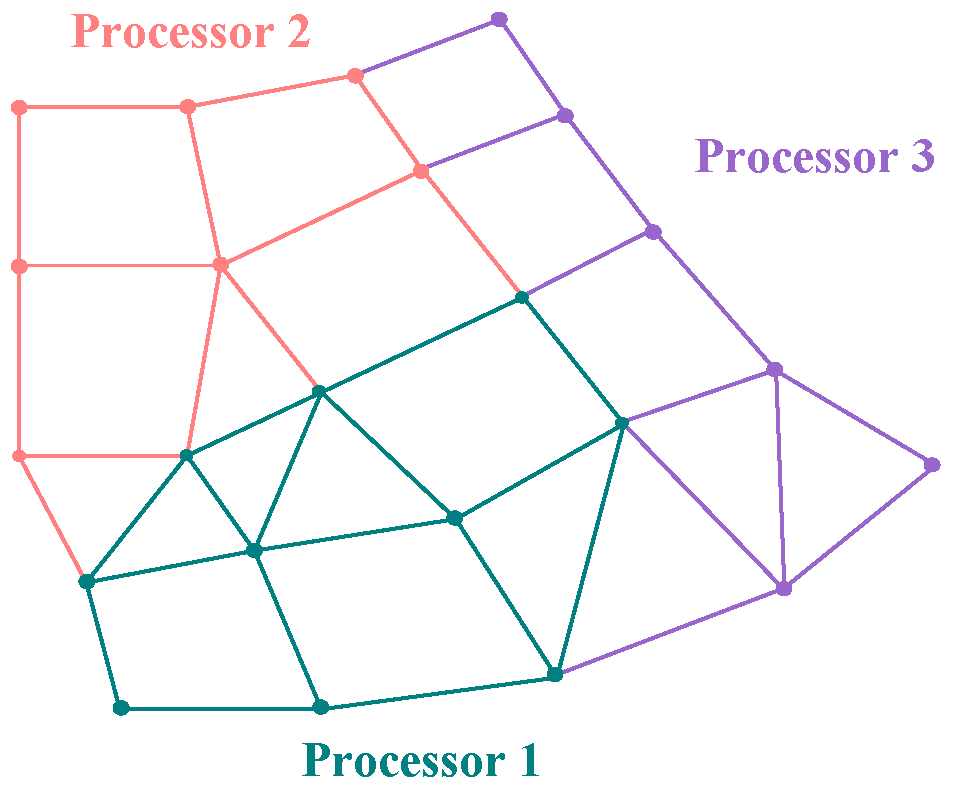
\includegraphics[width=.8\textwidth]{figures/data_structures/dof_distribution}
    \caption{Element and node ownership for an unstructured mesh partitioned into three subdomains.\label{fig:elem_node_ownership}}
  \end{center}
\end{figure}

Parallel degree of freedom indexing can then be performed using the approach outlined in Algorithm~\ref{alg:dof_indexing_parallel}. In this algorithm local degree of freedom indices are created for each processor in the range $[0,N_{dofs}^p)$.  All processes then broadcast the number of local degrees of freedom.  The global degree of freedom offset for each processor is then computed, and the global degree of freedom indices are given as $[N_{off}^p,N_{dofs}^p+N_{off}^p)$.
\begin{algorithm}[htbp]
  \centering
  \caption{Indexing degrees of freedom for the case when the mesh is parallelized across all processors.\label{alg:dof_indexing_parallel}}
   \begin{minipage}{.95\textwidth}
     \noindent
     \sffamily
     \setcounter{alines}{0}
     \begin{list}{\arabic{alines}:\ \ }{\usecounter{alines}}
       \renewcommand{\baselinestretch}{1.0} \setlength{\itemsep}{-1ex}
   	\item \textbf{for} $e=1$ to $N_{\text{local elements}}$ \textbf{do}
   	\item \ \ \ \textbf{for} $n=1$ to $N_{\text{element nodes}}$ \textbf{do}
   	\item \ \ \ \ \ \ \textbf{if} node is owned by $p$ and degrees of freedom are not indexed
   	\item \ \ \ \ \ \ \ \ \ index degrees of freedom
   	\item \ \ \ \ \ \ \textbf{endif}
   	\item \ \ \ \textbf{end}
   	\item \ \ \ index element degrees of freedom
   	\item \textbf{end}
   	\item gather the number of degrees of freedom for all processors $\{ N_{dofs}^p \}$
   	\item compute degree of freedom offset for processor $p$ as
   	  \begin{equation*}
   	    N_{off}^p=\sum_{i=1}^{p-1} N_{dofs}^i,\;\; p=2,3,\ldots,N_{\text{processors}}
   	  \end{equation*}
   	\item add offset to all local degree of freedom indices
     \end{list}
   \end{minipage}
\end{algorithm}

\subsection{Parallelizing the Adaptive Mesh Refinement Process}
The adaptive mesh refinement process involves the following steps:
\begin{enumerate}
  \tightlist
  \item Estimate the error in the solution and select elements for refinement and coarsening.
  \item Perform mesh refinement and coarsening.
  \item Project data from the old mesh onto the new mesh.
  \item Repartition and perform dynamic load balancing as necessary.
\end{enumerate}
Parallelization of the first step requires that the error estimator be locally computable on each subdomain.  This can be performed in a fashion similar to the local element computations performed in the matrix assembly phase.  The flux jump error indicator in Equation~\eqref{eqn:flux_indicator}, for example, is performed in parallel by computing contributions element-by-element for each subdomain.

Similarly, mesh refinement can occur in parallel with each processor performing refinement on its local elements.  The major concern in this step is that any new nodes added to the mesh are singly defined.  That is, care must be taken to ensure that new nodes on processor boundaries are not added twice.  This step may be performed by computing an identifying key for each node added and reconciling duplicate keys which may occur such that the topology of the refined mesh is consistent with the original mesh.

The local solution projection operators described in Section~\ref{sec:element_independent_amr} allow for the third step to be parallelized.  The required old mesh and corresponding solution data exist on each processor, and each processor will compute the projection onto the new elements (or restriction onto the coarsened mesh).  It is desirable to perform this step before any repartitioning of the mesh is performed because the data required for the projection step already reside local to the processor.  Therefore, in this approach the projection/restriction operators do not require inter-processor communication.

Finally, the refined mesh may no longer be well balanced across all processors.  In this case some repartitioning algorithm must be applied and some number of elements (and associated data) must be migrated between processors.  Note that this step has the highest communication overhead and therefore must be carefully implemented.  The repartitioning algorithm must strive to rebalance the mesh while requiring as little data migration as possible.  Diffusion-based algorithms are one method that can be used.  They attempt to rebalance the mesh by small changes in the location of the inter-processor boundaries, but this is not done here yet.

The particular architecture of a parallel machine may need to be considered when applying a repartitioning and load balancing algorithm.  In particular, on machines with very high bandwidth inter-processor interconnects it would likely be most beneficial to perform an optimal repartitioning such that the resulting mesh is well balanced.  This approach would trade load balancing for (relatively inexpensive) communication requirements.  Conversely, on a machine with a particularly low bandwidth interconnect the most efficient approach may be to accept additional computational load imbalance in order to avoid significant communication overhead incurred by an optimal repartitioning algorithm.

\subsection{Input/Output Considerations}
One potential bottleneck for parallel performance in any application is the input/output (I/O) process.  This is particularly true on parallel clusters composed of commodity machines as the I/O subsystem performance is often not optimized for simultaneous access by parallel processes. For modest problem sizes, the mesh I/O can be serialized through one processor without suffering a substantial performance hit because the underlying storage medium is the process bottleneck.

In the current implementation, the mesh is read in its entirety in serial by processor~1 and broadcast to all the other processors.  One immediate improvement to this process (which retains the serial read/write operation) is to read subsets of the mesh data structures in blocks and broadcast these blocks to all processors.  By using such a buffering process a mesh which is larger than the amount of physical memory available to any single processor may be used in a simulation, as each processor in general will require only a subset of the blocks in the mesh.  The current data structures could easily be generalized using this approach.  Each processor would then be required only to store its ``local'' elements and any adjacent elements which are connected via any node to these local elements.

Note that in this approach the \emph{entire} file containing the mesh is still read by one processor from disk in serial.  Memory limitations are overcome by essentially buffering the input stream, but the scalability of this approach is limited by its serial nature. An alternative procedure can be envisioned where each processor opens the file and seeks to its relevant location directly.  This approach works only in the case of a fast parallel file system which is required to avoid disk contention amongst the processors.  Alternate implementations are possible in which the mesh is preprocessed and subdivided into a number of individual files which correspond to each processor.  Again, note that the preprocessing step is likely to be serial.

In summary, there are a number of possibilities which exist for dealing with the scalability of I/O.  Many of these approaches are necessarily serial in one aspect or another.  This reflects the serial nature of the typical mesh generation $\rightarrow$ solution generation loop.  It is envisioned that in the future the proliferation of parallel mesh generation software could bypass this issue by coupling a parallel mesh generator directly to a parallel application code.

\subsection{Performance Expectations}
The parallelization strategy outlined above clearly imposes some additional overhead on certain fundamental library transactions, as is often the case in parallel algorithms.  That is to say, while a well-written parallel algorithm can always be run on a single processor, the implementation may not be optimal for this degenerate non-parallel case.

For this reason it is not suggested that the current, global mesh representation be abandoned outright and replaced with the parallel strategy outlined above.  Rather, the object-oriented design approach naturally supports multiple implementations of the underlying mesh technology with minimal impact on other portions of the library and no impact on external user code.

In this way a fully parallel implementation should be seen as an augmentation of current capabilities which may be used when it provides superior scalability or performance.  Previous experience with the global mesh model has shown reasonable scalability to modest numbers of processors.  Further, the global mesh approach vastly reduces much of the communication required during the adaptive mesh refinement process.  For this reason it is expected that, on particular parallel platforms, the current approach would likely outperform the fully parallel approach on a modest number of processors.  Of course, since the current implementation is not scalable, there will be a point at which the parallel implementation performance is superior.  However, this crossover point is necessarily platform dependent as it depends on the configuration of a given machine.  Therefore, the freedom to switch between the current global mesh approach and a fully parallel implementation should be maintained.

\section*{Summary}

This chapter discusses extensions of the data structures presented in Chapter~\ref{chap:amr} to allow for their efficient implementation on parallel computers.  A software implementation has been created in which a global representation of the mesh is stored on each processor and parallelization occurs at the matrix assembly, linear algebra, and error estimation levels.  A strategy for parallelizing the storage of the mesh and all associated aspects of the adaptive mesh refinement process was also presented.  The remaining chapters will apply the parallel adaptive technology discussed here to two distinct application classes.  

%% Local Variables:
%% TeX-master: "dissertation.tex"
%% End:

% LocalWords:  Discretization subdomains subdomain's subdomain AMR METIS MPI de
% LocalWords:  ParMETIS multithreading discretization Galerkin Krylov indices
% LocalWords:  rebalance benkirk endif dofs eqn
